% !TEX root = ../a2.tex

\section{Introduction}
In this report, we discuss the time complexity of three types of different selection algorithms including Randomized selection, Deterministic selection and Quick sorts, by testing their average runtime with input in different sizes. For each test case, every position will be tested as the order we want. The graph of time-size relationship, intuitively demonstrates the time complexity, thus confirming our theoretical expectation.

Since here we have to test each position as a test case, the time complexity for testing is raised to $O(n^2)$ and $O(n^2\log n)$ respectively. Thus, the maximum test case size is limited to $6\e{4}$, though the pattern is still clearly demonstrated.

\section{Performance analysis on Selection Algorithms}
\begin{figure}[H]
    \centering
    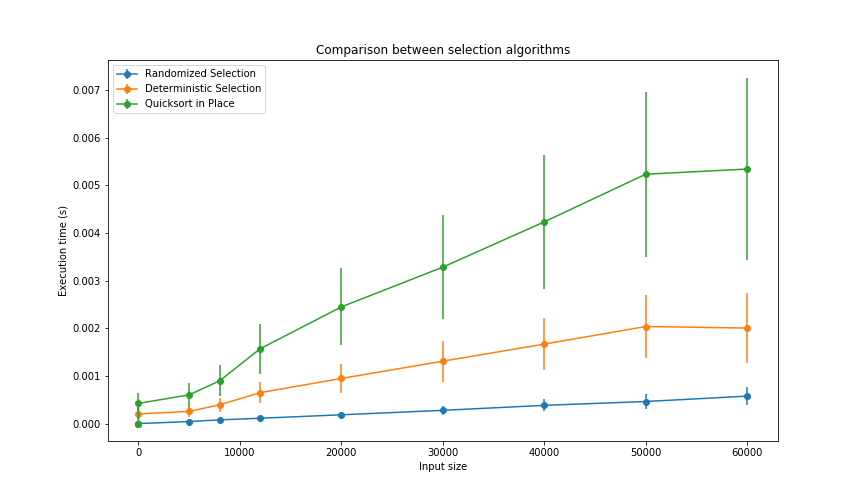
\includegraphics[width=0.75\linewidth]{../a2/test/res}
    \caption{Performance of selection algorithms}\label{res}
\end{figure}
To graphically demonstrate the outcome, here the standard deviation of tests are remained as error bar. The figure, as we expected, articulate a lower efficiency of the Quicksort solution.

Theoretically, in the worst case, Randomized selection will fail every time and degrade itself to the worst case of Quicksort, with time complexity $O(n^2)$. For Deterministic selection, the worst case is effectively restricted to $O(n)$ due to the \con{ChoosePivot} procedure.

For the two $O(n)$ selection algorithms, Randomized selection obtains a conspicuous advantage both on the runtime and standard deviation. Its little vibration indicates the stableness and reliability. In comparison, the uncertainty of Deterministic and Quicksort runtime is enormous.


\section{Conclusion}
In this report, we have demonstrated the characteristics of three different selection algorithms as well as their performance. Randomized selection is essentially the simplified version of Quicksort. Despite its unreliable worst case, it still obtains a better performance on average among these three algorithms. However, Deterministic selection makes a trade-off, which sacrifices its average performance for limiting its upper bound. In practice, it's sometimes worth a try and guarantees the steadiness of an entire procedure.

\clearpage
\section{Appendix}
\appendix
\section{Source Codes}
\inputcode{c++}{../a2/test/a2_test.cpp}{Three selection algorithms}{1}
\inputcode{python}{../a2/test/test.py}{Test case generator}{2}
\inputcode{bash}{../a2/test/test.sh}{Cases runner}{3}
\inputcode{python}{../a2/test/plot.py}{Plotting program}{4}